%\input{preamble}
%\begin{document}
\section{Definitions and notation}\label{sec:defs}
%\paragraph{Constraint systems}
In the following, a constraint system $S$ is a set of equalities and inequalities over the same set of variables, $\VAR(S)=\{x_1,\ldots, x_n\}$. 
Each constraint $c$ is either an equality, written $a_1x_1 + \ldots +a_nx_n = b$, or an inequality, written $a'_1x_1 + \ldots +a'_nx_n\leq b'$. Though, the left-hand-side is also written using a dot-product. 
%
We let $\var(c)$ denote the variables whose coefficient in $c$ is nonzero and say that $c$ \emph{uses} $x$ if $x\in \var(c)$.

The set of points in $\mathbb{R}^{|\VAR(S)|}$ that satisfies all constraints in $S$ is called $S$'s \emph{feasible area}. A constraint $c\in S$ is \emph{redundant} if it does not influence the feasible area for $S$. In other words the inequality $c: \ve{a}\cdot\ve{x}\leq b$ is redundant iff $\max \ve{a}\cdot\ve{x}$ w.r.t. $S\setminus\{c\}$ is less or equal to $b$.
An equality is redundant iff both corresponding inequalities are redundant.
If the constraint $c$ is \emph{not} redundant, it is called \emph{non-redundant} or binding.

%\paragraph{Projection}
As described above, the feasible area of $S$ is the combination of values for the variables in $\VAR(S)$ that satisfy all constraints in $S$. However, we assume that there are some variables $Y\subseteq \VAR(S)$ whose value in a feasible point we are not interested in; we just want to know that a satisfying value exists. This information is captured by the \emph{projection} of the feasible area of $S$ w.r.t. $Y$, $\mi{proj}_YS\in\mathbb{R}^{|\VAR(S)\setminus Y|}$. This is the largest set consisting of values for $\VAR(S)\setminus Y$ that can be extended with values for $Y$ such that all constraints in $S$ are satisfied (see Figure~\ref{fig:proj}). 

\begin{figure}
	\centering
		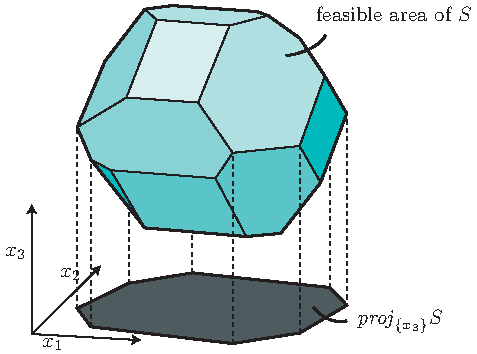
\includegraphics[scale=0.8]{figures/projection2.pdf}
	\caption{The projection of the system $S$ with respect to $\{x_3\}$.}
	\label{fig:proj}
\end{figure}

The projection of a system $S$ is a set of points in Euclidian space, and it is the feasible region of (another) system $S'$ (see e.g. \cite{ziegler95}). However, many constraint systems determine the same feasible area, and when we say e.g. ``$S'$ is the projection of $S$ w.r.t. $Y$'' we mean that ``$S'$ is one of the constraint systems whose feasible area equals the projection of the feasible area of $S$ w.r.t $Y$''.

%\paragraph{A note on $\VAR(S)$}
In this paper, we are mainly interested in the original system $S$ and its projection $S'$, while the associated feasible areas of $S$ and $S'$ are the ``mediator'' between the two systems. 
However, since the feasible area of a system is just a set of points in a multi-dimensional Euclidian space, the number and the order of the variables are important. However, to avoid unnecessarily heavy notation, in this paper we do not specify $VAR(S')$ formally for every considered constraint system $S$.
Intuitively, we just make sure that the dimensions (and order of variables) ``match''. For example, when two systems $T$ and $T'$ are joined to form another system $T''$, we consider $T$ and $T'$ as constraints over the same variable set, $VAR(T'')=var(T)\cup var(T')$.
A more stringent exposition keeping track of the variable sets and ordering can be found in \cite{MyTechRep}.
%\end{document}
